\begin{ccRefClass}{Tree_anchor<Data, Window>}

\ccDefinition
\ccStyle{Tree\_anchor} is also derived from
\ccStyle{Tree\_base}. Therefore, it provides the same
methods as
\ccStyle{Range\_tree\_d} and \ccStyle{Segment\_tree\_d},
but does nothing; it can be used as a
recursion anchor for those classes. Therefore,
instantiate \ccStyle{Sublayer\_type} of \ccStyle{Range\_tree\_d}
(\ccStyle{Segment\_tree\_d} respectively)
with \ccStyle{Tree\_anchor} and the container classes for
the data items (\ccStyle{Data} and \ccStyle{Window}).


\ccCreationVariable{a}
%\renewcommand{\ccAlternateThreeColumn}{\ccFalse}

\ccDefinition
\ccNestedType{Data}{container \ccStyle{Data}.}
\ccNestedType{Window}{container \ccStyle{Window}.}

\ccCreation
\ccInclude{CGAL/Tree_base.h}

\ccConstructor{Tree_anchor<Data, Window> a()}{}
%{saves all elements in a sequence container.}

%\renewcommand{\ccAlternateThreeColumn}{\ccTrue}
\ccOperations
\ccMethod{template<class OutputIterator>
OutputIterator window_query(Window win, OutputIterator result);}{~}
%{does nothing.}
%{pushes all elements to \ccStyle{result}.}

\ccMethod{template<class OutputIterator>
OutputIterator enclosing_query(Window win, OutputIterator result);}{~}
%{does nothing.}
%{pushes all elements to \ccStyle{result}.}

\ccMethod{bool is_valid();}{returns true;}

{\bf Protected Operations}

\ccMethod{bool is_inside(Window win,
  Data object);}{returns true.}

\ccMethod{bool is_anchor();}{returns true.}



%\vfill

%\pagebreak

\ccExample
The following figures show a number of rectangles and a $2$-dimensional 
segment tree built on them.

\begin{ccTexOnly}
\begin{figure}[htbp]
%\epsfxsize=12cm
%\centerline{\epsfbox{SearchStructures/segment_ex2.eps}}
    \begin{center}
    \includegraphics[width=12cm,clip]{segment_ex2.eps}
    \end{center}
\caption{\label{fig:rectangles}Two dimensional interval data.}
\end{figure}
\begin{figure}[htbp]
%\epsfxsize=12cm
%\centerline{\epsfbox{SearchStructures/segment_ex4.eps}}
    \begin{center}
    \includegraphics[width=12cm,clip]{segment_ex4.eps}
    \end{center}
\caption{\label{fig:segTreeEx}\protect Two dimensional segment tree
  according to the interval data of Figure~\ref{fig:rectangles}.}
\end{figure}
\end{ccTexOnly}
\begin{ccHtmlOnly}
        <!2><TABLE BORDER=0 CELLSPACING=2 CELLPADDING=0 WIDTH=650>
        <TR><TD ALIGN=LEFT VALIGN=TOP WIDTH=50% NOWRAP COLSPAN=2>
  <img border=0 src="./segment_ex2.gif" alt="Two
    dimensional interval data">
 </TD><<TD WIDTH=50%></TD><TD ALIGN=LEFT VALIGN=TOP
                           NOWRAP WIDTH=50%>
 <img border=0 src="./segment_ex4.gif" alt="Two
    dimensional segment tree according to the interval data"> </TD></TR>
        </TABLE><!2>

        <!2><TABLE BORDER=0 CELLSPACING=2 CELLPADDING=0 WIDTH=650>
        <TR><TD ALIGN=LEFT VALIGN=TOP WIDTH=50% NOWRAP COLSPAN=2>
Two dimensional interval data.
 </TD><TD WIDTH=50%></TD><TD ALIGN=LEFT VALIGN=TOP WIDTH=50%>
Two dimensional segment tree
  according to the interval data.
 </TD></TR>
        </TABLE><!2>
\end{ccHtmlOnly}
\end{ccRefClass}
